\documentclass[journal, letterpaper, 11pt]{IEEEtran}
\usepackage[utf8]{inputenc}
\usepackage[spanish]{babel}
\usepackage{amsmath}
\usepackage{amsfonts}
\usepackage{amssymb}
\usepackage{makeidx}
\usepackage{graphicx}
\usepackage{listings}
\usepackage{hyperref}
\usepackage{float}

\begin{document}
\title{Proyecto Bioinformática II\\Ensamble del genoma de \textit{pseudomonas aeruginosa}}
\author{Salvador~Alejandro~Cuevas~Villicaña,~\IEEEmembership{Ciencias~Agrogenómicas}
\thanks{Estudiante de segundo año de la licenciatura en Ciencias Agrogenómicas en la Escuela Nacional de Estudios Superiores Unidad León de la Universidad Nacional Autónoma de México, (e-mail: alejandro.villicana@comunidad.unam.mx)} 
}

\markboth{Semestre~2022-1, Fecha~de~entrega~6~de~Diciembre~del~2021}
{Shell \MakeLowercase{\textit{et al.}}: Bare Demo of IEEEtran.cls for IEEE Journals}

\maketitle

\begin{abstract}
\textit{Pseudomonas aeruginosa} es una bacteria ubicua ambiental, gram-negativa que pertenece a la rama $\gamma$ de las proteo-bacterias, y es una de las principales causantes de enfermedades oportunistas en animales y plantas; causando en los humanos infecciones en las vías respiratorias, urinarias y tejidos. Esta posición se le debe principalmente a su elevada resistencia a los antibióticos y desinfectantes. Este trabajo presenta el ensamble de un genoma público de \textit{P. aeruginosa} secuenciado mediante la tecnología de Illumina MiSeq, desde como descargar las secuencias hasta la anotación del ensamble de las mismas. Mediante el uso de varias herramientas bioinformaticas
\end{abstract}


\begin{IEEEkeywords}
\textit{P. aeruginosa}, bioinformática, genoma, Illumina MiSeq, ensamble, anotación de secuencias
\end{IEEEkeywords}

\IEEEpeerreviewmaketitle



\section{Introducción}

\IEEEPARstart{L}{a} bacteria \textit{Pseudomonas aeruginosa} es una especie de relevancia tanto medica como en actividades agro-productivas. Ya que es la causante de varias enfermedades oportunistas en plantas y animales. Es gram-negativa, aerobia, suele habitar en ecosistemas húmedos, así como en plantas y tejidos vegetales. Las infecciones que suelen afectar al sistema respiratorio, el sistema urinario, y a heridas abiertas causando sepsis. Estas infecciones son imposibles de erradicar, en parte debido a la resistencia natural de la bacteria a los antibióticos, y en última instancia conducen a insuficiencia pulmonar y muerte.

Tiene un genoma significativamente grande que, a comparación de otras bacterias, con un tamaño de 6,3 millones pares de bases (Mbp), la secuenciación y ensamble de su genoma en teoría  permitiría encontrar nuevas alternativas para luchas contra sus infecciones.

\subsection{Ensamble de genomas}
Los archivos obtenidos de una secuenciación contienen millones de fragmentos de ADN que no tienen una utilidad de estudio. Por lo que hace falta ensamblar esos millones de fragmentos en un Genoma completo. Es un proceso complejo que demanda muchas prestaciones computacionales. Existen dos tipos de ensamble de genoma: de novo y ensambles de referencia; los primeros se realizan cuando no se tiene otro genoma ensamblado para poder compararlo y el ensamble de referencia es cuando se realiza hacia un genoma previamente ensamblado. Ambas estrategias presentan sus pros y contras; pero de cualquier forma el procedimiento a seguir es muy similar y consta de los siguientes pasos:

\begin{itemize}
\item Control de calidad. Donde se verifica si nuestros archivos de secuenciación son viables para realizar un ensamble y que tan contaminados se encuentran,
\item Filtrado. Si vemos que son viable los archivos. Se realiza un filtrado para eliminar adaptadores de secuenciación y secuencias parasitas.
\item Calculo de Cobertura. De la secuenciación
\item Si existe una referencia previa se puede realizar un mapeo.
\item El ensamble del genoma. Existen varias herramientas y el cual usar depende de si se usara una estrategia de novo o de referencia.
\item Anotación. Una vez teniendo nuestro genoma ensamblado. Se procede a realizarle la anotación donde se le añade la información biológica relevante; la anotación se divide en estructural y funcional, la estructural es definir la región donde se encuentran los genes en el genoma y la funcional es la función que cumplen estos genes en el organismo.
\end{itemize}

\section{Metodología}
Se usaron varias herramientas bioinformáticas, la mayoría de software libre, la mayoría de los cuales se ejecutaron mediante el protocolo SSH en el clúster denominado “GAIA” perteneciente a la Escuela Nacional de Estudios Superior Unidad León de la UNAM, y otro en mi propio ordenador personal con las siguientes prestaciones:

\begin{itemize}
\item Procesador: Intel(R) Core(TM) i7-9750H CPU @ 2.60GHz   2.59 GHz
\item RAM instalda: 16 GB
\item Sistema operativo: Windows 11 Home con WSL2 que corre Ubuntu 20.04 lts
\end{itemize}

Así mismo también se usó la base de datos del NCBI \linebreak

\subsubsection{Descarga de secuencias del NCBI}
\textbf{Se uso GAIA.} Mediante la herramienta SRAtoolkit \url{https://trace.ncbi.nlm.nih.gov/Traces/sra/sra.cgi?view=toolkit_doc} previamente instalada en GAIA, se procedió a descargar la secuencia marcada con el indicador SRR17084738, mediante el comando:

\lstset{breaklines=true, basicstyle=\footnotesize}
\begin{lstlisting}[frame=single]
fastq-dump --split-3 SRR17084738
\end{lstlisting}

La opción --split-3 nos sirve para bajar secuencias pareadas, como es en el caso de ésta. Con este comando se obtuvieron los archivos SRR17084738\_1 y SRR17084738\_2 de la secuencia pareada de \textit{P. aeruginosa}
\linebreak
\subsubsection{Control de calidad}
\textbf{Se uso GAIA.} El primer análisis de control de calidad se realizó mediante FASTQC, \url{https://www.bioinformatics.babraham.ac.uk/projects/fastqc/}, previamente instalado en GAIA, el comando que usé es:

\lstset{breaklines=true, basicstyle=\footnotesize}
\begin{lstlisting}[frame=single]
fastqc SRRSRR17084738*
\end{lstlisting}

Obteniendo como resultado los reportes html de FASTQC, donde se observó que la muestra estaba contaminada por el adaptador "nextera transposase sequence" y un tamaño total de 1,024,419 secuencias. Por lo que el siguiente paso fue eliminar las secuencias de adaptadores, otros adaptadores y secuencias de baja calidad.
\linebreak
\subsubsection{Filtrado de secuencias}
\textbf{Se uso GAIA.}Para el filtrado de secuencias use FASTP \url{https://github.com/OpenGene/fastp}, previamente instalado en GAIA, este se realiza a las secuencias que se obtuvieron en el punto II-1 y mediante el comando:

\lstset{breaklines=true, basicstyle=\footnotesize}
\begin{lstlisting}[frame=single]
fastp -i SRR17084738_1.fastq -I SRR17084738_2.fastq -o filtrado_1.fastq -O filtrado_2.fastq --qualified_quality_phred 30
\end{lstlisting}

La opción elegidas para este comando fue establecer que las secuencias no podían bajar de un nivel de calidad phred 30 mediante --qualified\_quality\_phred 30; la escala phred nos indica la calidad de nuestra secuenciación  mediante la probabilidad de factor de error de cada base, determinada por la ecuación matemática $P=10^{\dfrac{-Q}{10}}$, siendo $Q $ el nivel de calidad phred y $P$ la probabilidad de factor de error de base. Por lo que para un nivel calidad 30, la probabilidad de obtener un error es de 1 en 1000 bases. \linebreak Una vez realizado el filtrado se obtuvieron los archivos filtrado\_1.fastq y filtrado\_2.fastq ; a los cuales se le realizo nuevamente un FASTQC para comprobar las nuevas calidades. Esto es mediante:

\lstset{breaklines=true, basicstyle=\footnotesize}
\begin{lstlisting}[frame=single]
fastqc filtrado_*
\end{lstlisting}

Una vez realizado el nuevo análisis se comprobó que se habían eliminado los adaptadores y que un 74.802107\% de las secuencias habían pasado el filtrado de calidad, es decir 766,287 secuencias que tienen un score phred mayor a 30 \linebreak
\subsubsection{Cálculo de cobertura}
\textbf{Se uso GAIA.}
Para el calculo de cobertura se usaron los siguientes comandos a los archivos filtrado\_1.fastq y filtrado\_2.fastq 

\lstset{breaklines=true, basicstyle=\footnotesize}
\begin{lstlisting}[frame=single]
cat filtrado_1.fastq | paste - - - - | awk '{print$2}' | wc -l
\end{lstlisting}

Cuyo resultado es 766287, es decir el numero total secuencias.

\lstset{breaklines=true, basicstyle=\footnotesize}
\begin{lstlisting}[frame=single]
cat filtrado_1.fastq | paste - - - - | awk '{print$2}' | wc -c
\end{lstlisting}

Y su resultado es el numero de saltos de linea.\linebreak Finalmente el resultado de la cobertura es el restar el segundo valor menos el primero.

\[5300155 - 766287 = 4533868\]

Es decir la cobertura tiene un valor de $4533868$

Se obtiene el mismo resultado con el archivo filtrado\_2.fastq 
\linebreak
\subsubsection{Mapeo}
\textbf{Se uso GAIA.}
Se realizó un mapeo a referencia mediante la herramienta bowtie2, \url{http://bowtie-bio.sourceforge.net/bowtie2/index.shtml} , previamente instalada en GAIA, por lo que primero se descargó una secuencia de referencia en el NCBI, eligiendo la que tiene el identificador NC\_002516.2 "Pseudomonas aeruginosa PAO1, complete genome" almacenado locamente como $refgenome.fasta$ 

Luego se realizó el indice con el comando:

\lstset{breaklines=true, basicstyle=\footnotesize}
\begin{lstlisting}[frame=single]
bowtie2-build -f refgenome.fasta REFpsea
\end{lstlisting}

Luego el mapeo se realiza con:

\lstset{breaklines=true, basicstyle=\footnotesize}
\begin{lstlisting}[frame=single]
bowtie2 -S filtradovsPsea.sam -q --phred33 -p 4 --fr -x  REFpsea -1 filtrado_1.fastq -2 filtrado_2.fastq >& bowtie_psea.log
\end{lstlisting}

Obteniendo el archivo de mapeo $filtradovsPsea.sam$ al cual se le eliminaran las secuencias que no mapearon mediante el comando:

\lstset{breaklines=true, basicstyle=\footnotesize}
\begin{lstlisting}[frame=single]
awk $3!="*" filtradovsPsea.sam >filtradovsREF_reducido.sam
\end{lstlisting}

Obteniendo finalmente el archivo $filtradovsREF\_reducido.sam$ 
\linebreak
\subsubsection{Ensamble de genomas}
\textbf{Se uso GAIA.}
Para el ensamble del genoma se usó el programa SPAdes, \url{https://github.com/ablab/spades} ,previamente instalado en GAIA. El ensamble se realizó con el comando:

\lstset{language=Python,breaklines=true, basicstyle=\footnotesize}
\begin{lstlisting}[frame=single]
spades.py -k 21,33,37,41,55,77 -t 4 -m 8 --pe1-1 filtrado_1.fastq --pe1-2 filtrado_2.fastq -o spades_Psea
\end{lstlisting}

Las opciones usadas son  -k 21,33,37,41,55,77 que indican los valores de tamaños k-mer que se utilizarán, -t 4 que indica el número de hilos, 4 en este caso, -m que indica el número máximo de memoria RAM que puede usar SPAdes, 8GB en este caso y --pe1-1 y --pe1-2 que indica cual es el archivo 1 y el 2 respectivamente del pareo.

Posteriormente se realiza un análisis de calidad del ensamble mediante el archivo scaffolds.fasta generado y es mediante el comando:

\begin{lstlisting}[frame=single]
quast --split-scaffolds -t 1 scaffolds.fasta
\end{lstlisting}

Posteriormente se realiza una análisis de calidad hacia el genoma de referencia. Mediante el comando:

\begin{lstlisting}[frame=single]
quast.py --split-scaffolds -t 1 -r refgenome.fasta scaffolds.fasta
\end{lstlisting}

\subsubsection{Anotación}
\textbf{Se uso PC}
Una vez teniendo los resultados del ensamble se procede a separar los scaffolds que estan en el archivo scaffolds.fasta para poder realizar la anotación estructural y funcional del mismo. Solo se realizó la preperación del primero porque el porcedimineto es igual para los demas. Y para esto me apoye en la pagina FAS Center dor Systems Biology \url{http://archive.sysbio.harvard.edu/CSB/resources/computational/scriptome/UNIX/Tools/Change.html}

Primero se pasa el archivo `scaffolds.fasta` a formato tabular mediante el comando:

\begin{lstlisting}[frame=single]
perl -e ' $count=0; $len=0; while(<>) { s/\r?\n//; s/\t/ /g; if (s/^>//) { if ($. != 1) { print "\n" } s/ |$/\t/; $count++; $_ .= "\t"; } else { s/ //g; $len += length($_) } print $_; } print "\n"; warn "\nConverted $count FASTA records in $. lines to tabular format\nTotal sequence length: $len\n\n"; ' scaffolds.fasta > scaffolds.tab
\end{lstlisting}

Luego se calcula la longitud de la última columna de `scaffolds.tab` que es la longitud del scaffolds

\begin{lstlisting}[frame=single]
perl -e ' $col=-1; while (<>) { s/\r?\n//; @F = split /\t/, $_; $len = length($F[$col]); print "$_\t$len\n" } warn "\nAdded column with length of column $col for $. lines.\n\n"; ' scaffolds.tab > seqs_length.tab 
\end{lstlisting}

Luego se corta esa última columna que nos indica el valor numérico de la longitud del scaffols, mediante el comando:

\begin{lstlisting}[frame=single]
cut -f 4 seqs_length.tab > onlylength.list
\end{lstlisting}

Luego para ver la longitud de los scaffold que tenemos usamos el comando:


\begin{lstlisting}[frame=single]
cat onlylength.list | more
\end{lstlisting}

Elegí el primero, el que tiene longitud de $668648$

Ahora para ver la nomenclatura de estos scaffolds para poder sepáralos del resto, se usa el comando:

\begin{lstlisting}[frame=single]
head -n 1 seqs_length.tab | cut -f 1.
\end{lstlisting}

Dando como resultado que el primer scaffold se llama: \textbf{NODE\_1\_length\_668648\_cov\_39.096881}

Luego se genera una lista donde se almacena el nombre del scaffold para poder separarlo del resto de los demás:

\begin{lstlisting}[frame=single]
vim SCA1.list
\end{lstlisting}

Luego se realiza el recorte del scaffold con el comando:

\begin{lstlisting}[frame=single]
perl -e ' ($id,$fasta)=@ARGV; open(ID,$id); while (<ID>) { s/\r?\n//; /^>?(\S+)/; $ids{$1}++; } $num_ids = keys %ids; open(F, $fasta); $s_read = $s_wrote = $print_it = 0; while (<F>) { if (/^>(\S+)/) { $s_read++; if ($ids{$1}) { $s_wrote++; $print_it = 1; delete $ids{$1} } else { $print_it = 0 } }; if ($print_it) { print $_ } }; END { warn "Searched $s_read FASTA records.\nFound $s_wrote IDs out of $num_ids in the ID list.\n" } ' SCA1.list scaffolds.fasta > scaffold_NODE_1.fna
\end{lstlisting}

Ahora teniendo nuestro scaffold NODE\_1 se procedió a realizar la anotación estructural y esto es mediante la interfaz web de augustus \url{https://bioinf.uni-greifswald.de/augustus/} . Como parametros se eligió: organismo de referencia a \textit{Escherichia Coli}, Report genes en both strands y Alternative transcripts en middle

Luego de analizar la parte gráfica del reporte de Augustus se opto por elegir los genes g401.t1 al g425.t1 para realizar la anotación funcional. Y para esto de la sección de predicted amino acid sequences y predictes coding sequences del mismo reporte de Agustus se extrajeron dichas secuencias almacenándose en archivos .faa y .fna respectivamente. 

Posteriormente para la antoación funcional se uso la herramienta blast del NCBI donde se obtuvieron porcentajes de identidad del 99 \% al 100\% en los 26 genes estudiados para el caso del archivo de nucleotidos.fna que se corrió contra la base de datos de non-redundant protein sequences (nr) con los demas valores por default y un 90 \% al 100\% de identidad con el archivo aminoacidos.faa  y que se corrió con la base de datos de nucleotide collection (nr/nt) y los demás valores por default.

Finalmente se uso el softwere propietario Blast2Go \url{https://www.blast2go.com/} en su versión basica para comparar ambos resultados unicamente al arhcivo aminoacidos.faa y donde 6 de los genes estudiados completaron el proceso de anotación

\section{Resultados}
Esta sección contiene los resultados detallados de los procedimientos realizados en la sección "II. Metodología" \linebreak
\subsubsection{Descarga de secuencias del NCBI}
La información del genoma usado es:

\begin{itemize}
\item Size: 282.1Mb
\item Instrument: Illumina MiSeq
\item Strategy: WGS
\item Source: GENOMIC 
\item Selection: RANDOM
\item Layout: PAIRED
\end{itemize}
Al ejecutar el comando de descarga se obtienen dos archivos de 579.899 MB cada uno denominados SRR17084738\_1 y SRR17084738\_2 , los cuales contienen el genoma dividido en cada uno de sus pares. \linebreak

\subsubsection{Control de calidad}
Los resultados del FASTQC de cada uno de los pares son los siguientes:
\begin{figure}[H]
\centering
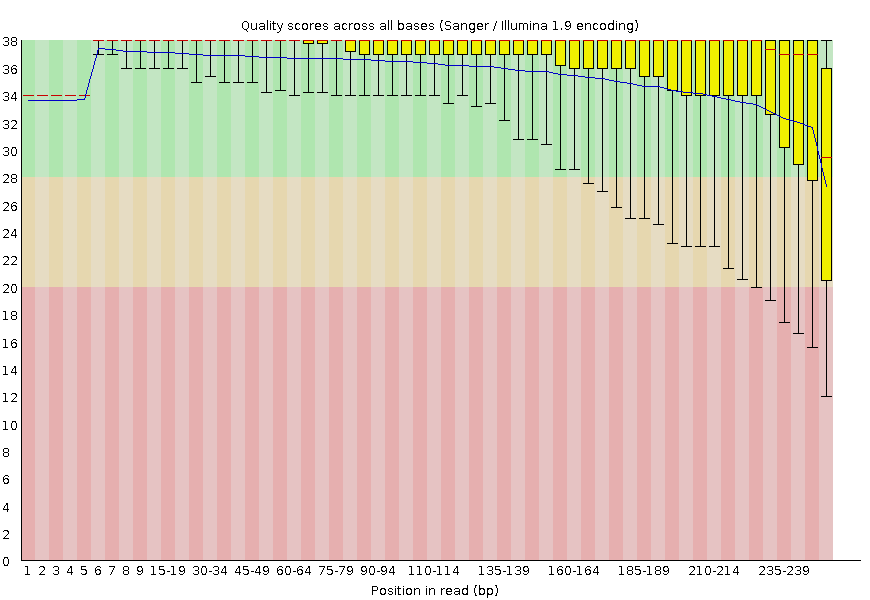
\includegraphics[width=7cm]{Imagenes/fastqc_original_1_2.png}
\caption{Calidad de SRR17084738\_1}
\end{figure}
\begin{figure}[H]
\centering
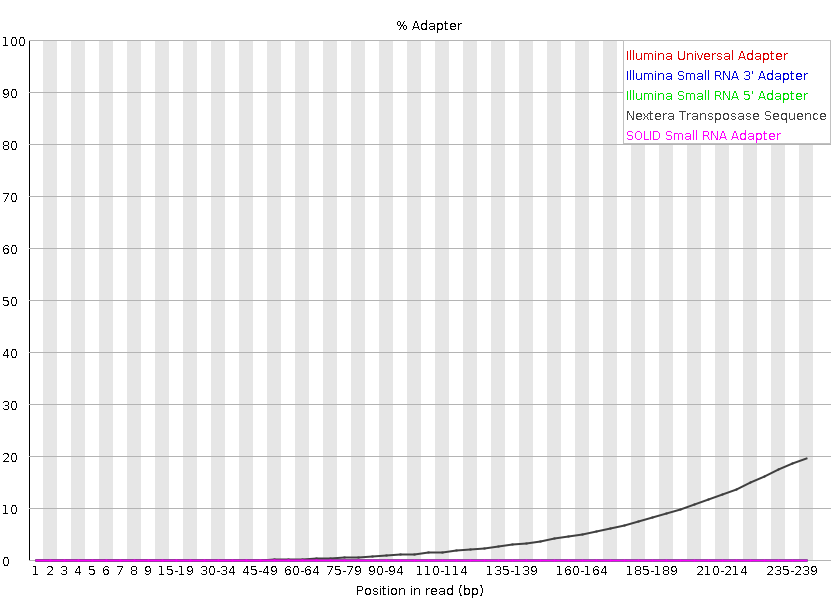
\includegraphics[width=7cm]{Imagenes/fastqc_original_1_1.png}
\caption{Contaminante de adaptadores SRR17084738\_1}
\end{figure}

\begin{figure}[H]
\centering
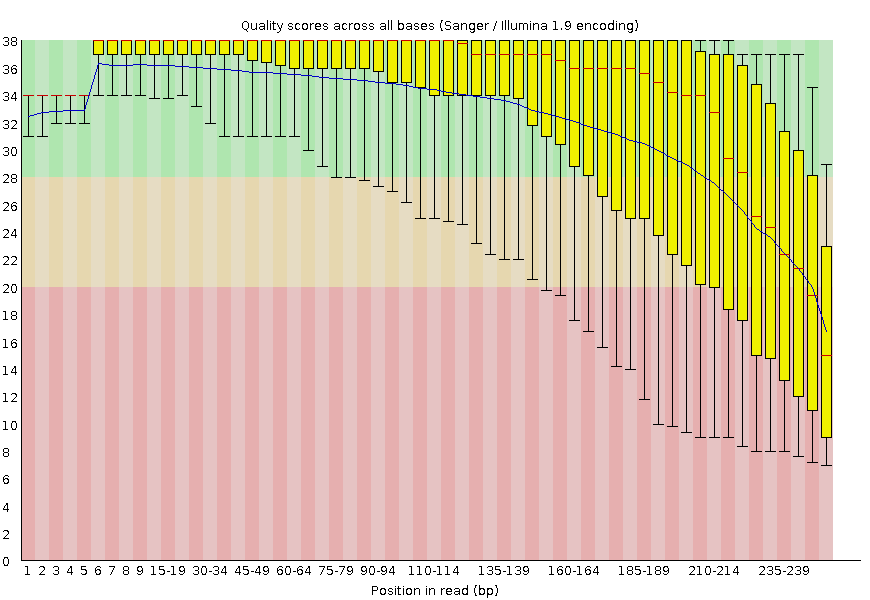
\includegraphics[width=7cm]{Imagenes/fastqc_2_1.png}
\caption{Calidad de SRR17084738\_2}
\end{figure}
\begin{figure}[H]
\centering
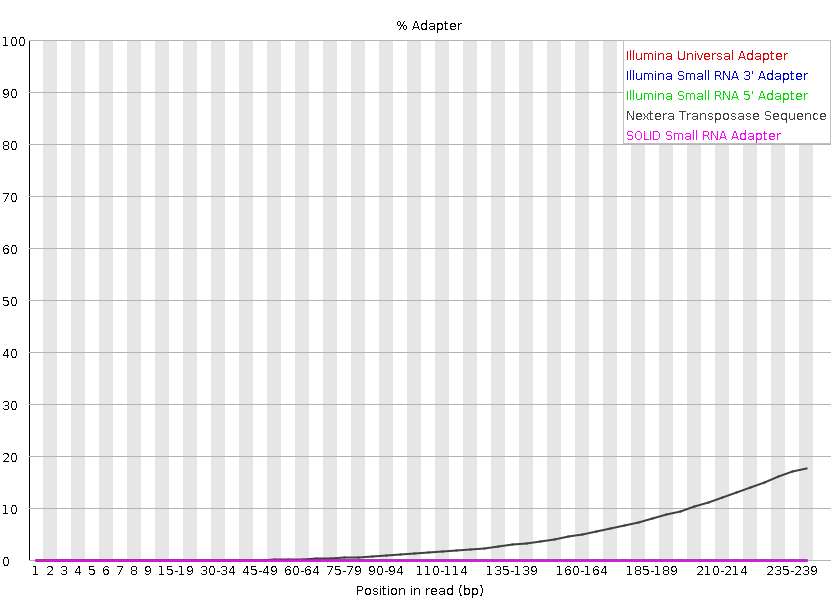
\includegraphics[width=7cm]{Imagenes/fastqc_2_2.png}
\caption{Contaminante de adaptadores SRR17084738\_2}
\end{figure}



Lo más destacable al respecto es que:

\begin{itemize}
\item Tamaño total: 1,024,419 secuencias
\item \%GC : 65, mas que el porcentaje teoríco
\end{itemize}

También el FastQC arrojó que la muestra estaba contaminada con el adaptador "nextera transposase sequence", por lo que el siguiente paso fue realizar un filtrado de secuencias \linebreak


\subsubsection{Filtrado de secuencias}
Después de realizar un análisis de FASTQC al resultado del filtrado de FASTP condicionado a una calidad phred mayor a 30 se obtuvieron los siguientes resultados:

\begin{figure}[H]
\centering
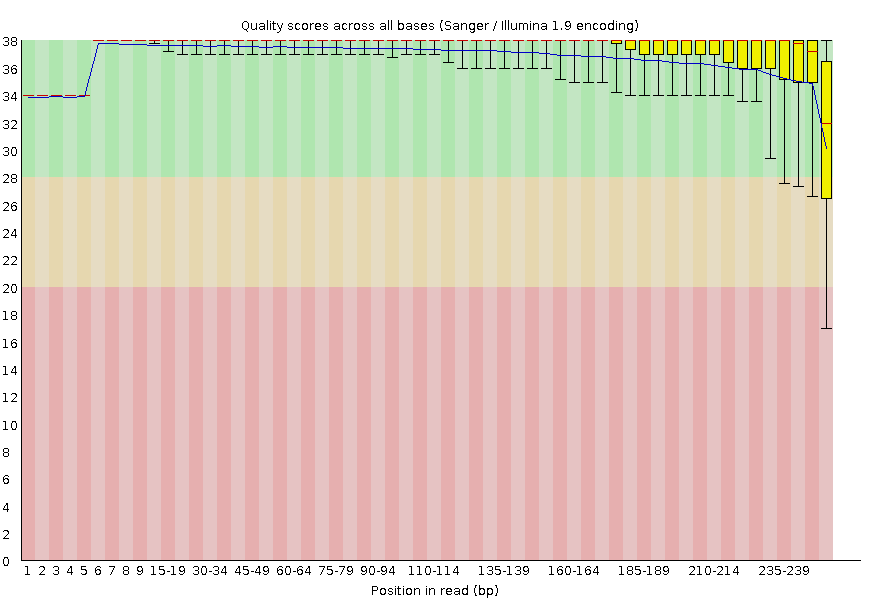
\includegraphics[width=7cm]{im_filtrado/2_2.png}
\caption{Calidad de filtrado\_1}
\end{figure}
\begin{figure}[H]
\centering
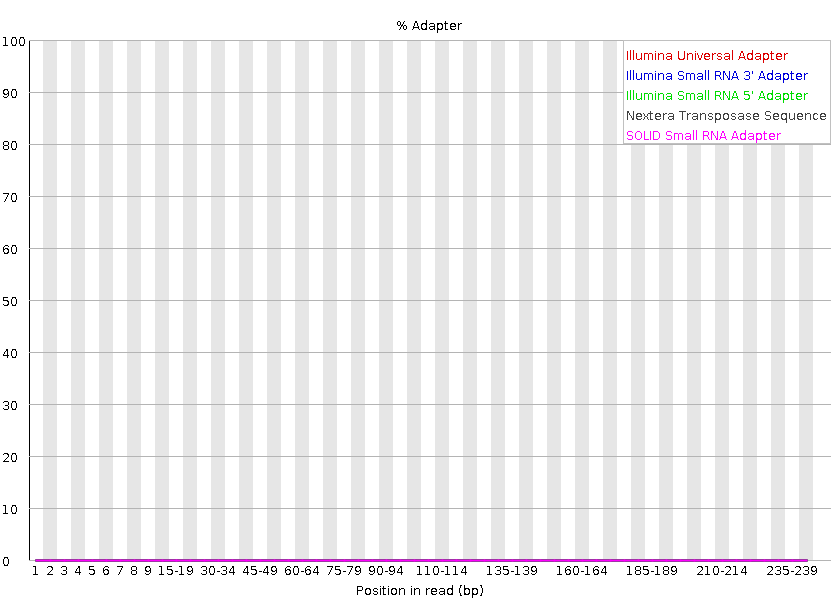
\includegraphics[width=7cm]{im_filtrado/1_1.png}
\caption{Contaminante de adaptadores de filtrado\_1}
\end{figure}
\begin{figure}[H]
\centering
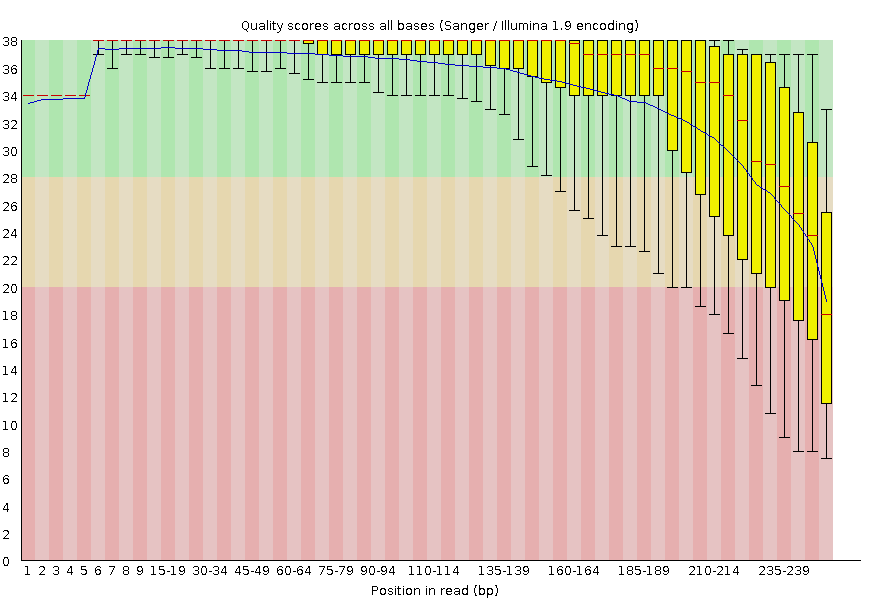
\includegraphics[width=7cm]{im_filtrado/3_1.png}
\caption{Calidad de filtrado\_2}
\end{figure}
\begin{figure}[H]
\centering
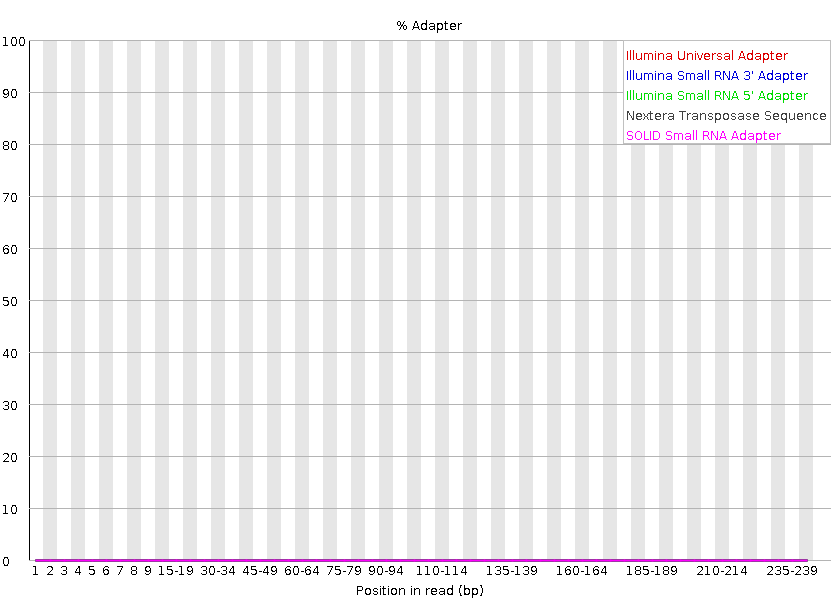
\includegraphics[width=7cm]{im_filtrado/3_2.png}
\caption{Contaminante de adaptadores de filtrado\_2}
\end{figure}

Del total de secuencias originales solo 766,287 pasaron el filtrado, es decir únicamente 74.802107\% de ellas, asi mismo se logro eliminar los adaptadores de ambos archivos

\subsubsection{Cálculo de cobertura}
Aquí se muestra la ejecución de los comandos por los cuales se llega al valor de la cobertura.
\begin{figure}[H]
\centering
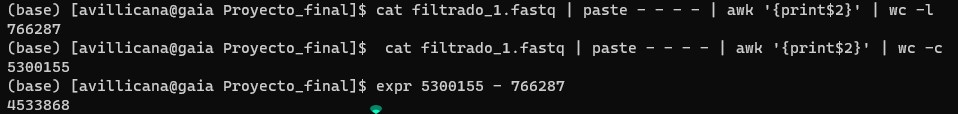
\includegraphics[width=9cm]{imagenes/cobertura.png}
\caption{Calculo de cobertura}
\end{figure}
Dando como resultado el valor de $4533868$ para la cobertura \linebreak

\subsubsection{Mapeo}
Las primeras lineas del mapeo sin las secuencias que no mapearon son:

\begin{figure}[H]
\centering
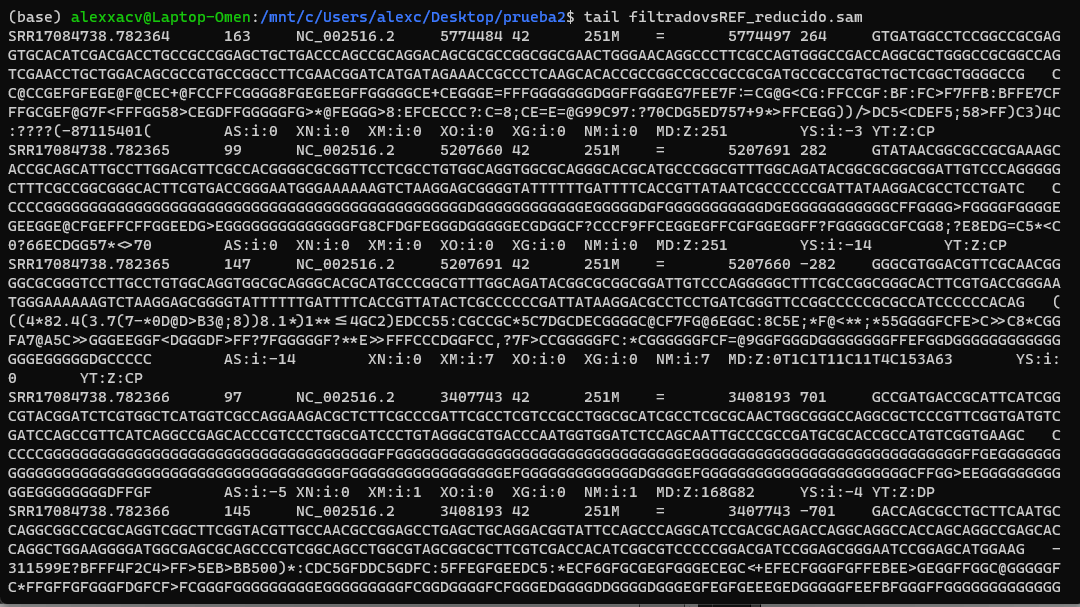
\includegraphics[width=9cm]{imagenes/mapeoreducido.png}
\caption{Primeras lineas del mapeo reducido}
\end{figure}


\subsubsection{Ensamble de genomas}
En el análisis sin referencia tenemos:

\begin{table}[H]
\begin{center}
\caption{Reporte calidad de mapeo sin referencia. All statistics are based on contigs of size $\geq$ 500 bp, unless otherwise noted (e.g., "\# contigs ($\geq$ 0 bp)" and "Total length ($\geq$ 0 bp)" include all contigs).}
\begin{tabular}{|l*{2}{|r}|}
\hline
Assembly & scaffolds & scaffolds\_broken \\ \hline
\# contigs ($\geq$ 0 bp) & 80 & - \\ \hline
\# contigs ($\geq$ 1000 bp) & 48 & 57 \\ \hline
\# contigs ($\geq$ 5000 bp) & 41 & 50 \\ \hline
\# contigs ($\geq$ 10000 bp) & 38 & 47 \\ \hline
\# contigs ($\geq$ 25000 bp) & 34 & 41 \\ \hline
\# contigs ($\geq$ 50000 bp) & 30 & 35 \\ \hline
Total length ($\geq$ 0 bp) & {\bf 6425745} & - \\ \hline
Total length ($\geq$ 1000 bp) & {\bf 6414820} & 6413920 \\ \hline
Total length ($\geq$ 5000 bp) & {\bf 6403294} & 6402394 \\ \hline
Total length ($\geq$ 10000 bp) & {\bf 6385298} & 6384398 \\ \hline
Total length ($\geq$ 25000 bp) & {\bf 6321690} & 6286931 \\ \hline
Total length ($\geq$ 50000 bp) & {\bf 6171899} & 6075814 \\ \hline
\# contigs & 55 & 64 \\ \hline
Largest contig & 668648 & 668648 \\ \hline
Total length & {\bf 6419571} & 6418671 \\ \hline
GC (\%) & 66.39 & 66.39 \\ \hline
N50 & {\bf 303720} & 239845 \\ \hline
N75 & {\bf 160338} & 106343 \\ \hline
L50 & {\bf 7} & 9 \\ \hline
L75 & {\bf 14} & 19 \\ \hline
\# N's per 100 kbp & 14.02 & {\bf 0.00} \\ \hline
\end{tabular}
\end{center}
\end{table}

\begin{figure}[H]
\centering
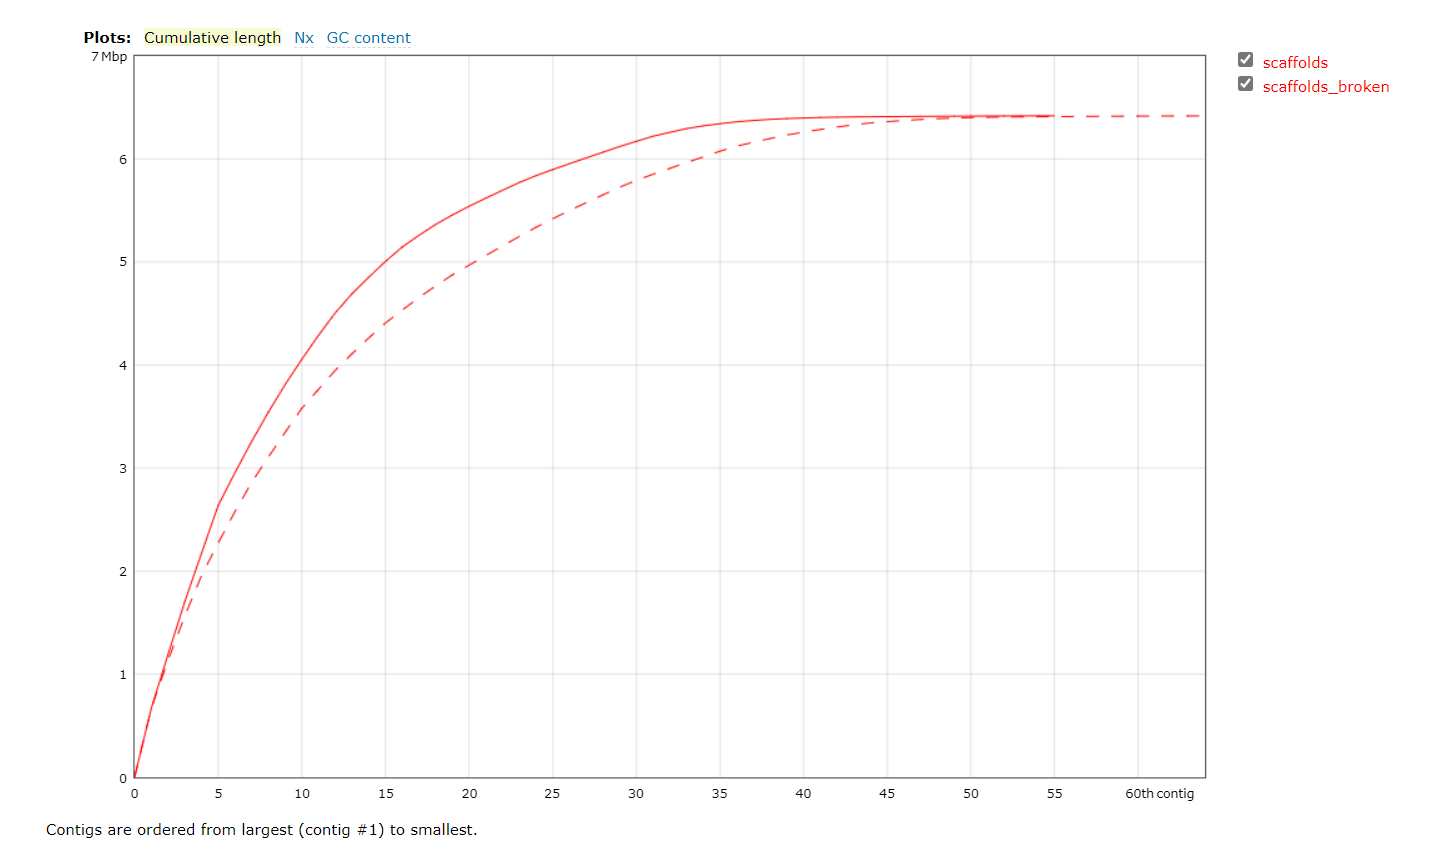
\includegraphics[width=9cm]{imagenes/mapeosin.png}
\caption{Gráfica de longitud acumulativa de la calidad sin referencia}
\end{figure}

En el análisis con referencia tenemos:

\begin{table}[H]
\begin{center}
\caption{Reporte calidad de mapeo con referencia. All statistics are based on contigs of size $\geq$ 500 bp, unless otherwise noted (e.g., "\# contigs ($\geq$ 0 bp)" and "Total length ($\geq$ 0 bp)" include all contigs).}
\begin{tabular}{|l*{2}{|r}|}
\hline
Assembly & scaffolds & scaffolds\_broken \\ \hline
\# contigs ($\geq$ 0 bp) & 80 & - \\ \hline
\# contigs ($\geq$ 1000 bp) & 48 & 57 \\ \hline
\# contigs ($\geq$ 5000 bp) & 41 & 50 \\ \hline
\# contigs ($\geq$ 10000 bp) & 38 & 47 \\ \hline
\# contigs ($\geq$ 25000 bp) & 34 & 41 \\ \hline
\# contigs ($\geq$ 50000 bp) & 30 & 35 \\ \hline
Total length ($\geq$ 0 bp) & {\bf 6425745} & - \\ \hline
Total length ($\geq$ 1000 bp) & {\bf 6414820} & 6413920 \\ \hline
Total length ($\geq$ 5000 bp) & {\bf 6403294} & 6402394 \\ \hline
Total length ($\geq$ 10000 bp) & {\bf 6385298} & 6384398 \\ \hline
Total length ($\geq$ 25000 bp) & {\bf 6321690} & 6286931 \\ \hline
Total length ($\geq$ 50000 bp) & {\bf 6171899} & 6075814 \\ \hline
\# contigs & 55 & 64 \\ \hline
Largest contig & 668648 & 668648 \\ \hline
Total length & {\bf 6419571} & 6418671 \\ \hline
Reference length & 6264404 & 6264404 \\ \hline
GC (\%) & 66.39 & 66.39 \\ \hline
Reference GC (\%) & 66.56 & 66.56 \\ \hline
N50 & {\bf 303720} & 239845 \\ \hline
NG50 & {\bf 303720} & 239845 \\ \hline
N75 & {\bf 160338} & 106343 \\ \hline
NG75 & {\bf 160338} & 113612 \\ \hline
L50 & {\bf 7} & 9 \\ \hline
LG50 & {\bf 7} & 9 \\ \hline
L75 & {\bf 14} & 19 \\ \hline
LG75 & {\bf 14} & 18 \\ \hline
\# misassemblies & 43 & {\bf 42} \\ \hline
\# misassembled contigs & 20 & 20 \\ \hline
Misassembled contigs length & 5108685 & {\bf 4067034} \\ \hline
\# local misassemblies & 42 & 42 \\ \hline
\# scaffold gap ext. mis. & {\bf 1} & - \\ \hline
\# scaffold gap loc. mis. & {\bf 6} & - \\ \hline
\# unaligned mis. contigs & 0 & 0 \\ \hline
\# unaligned contigs & {\bf 1 + 26 part} & 1 + 27 part \\ \hline
Unaligned length & 403575 & {\bf 403122} \\ \hline
Genome fraction (\%) & {\bf 95.939} & 95.937 \\ \hline
Duplication ratio & 1.001 & 1.001 \\ \hline
\# N's per 100 kbp & 14.02 & {\bf 0.00} \\ \hline
\# mismatches per 100 kbp & 493.93 & {\bf 493.79} \\ \hline
\# indels per 100 kbp & 10.48 & {\bf 10.45} \\ \hline
Largest alignment & {\bf 389953} & 389622 \\ \hline
Total aligned length & {\bf 6014261} & 6014061 \\ \hline
NA50 & {\bf 125560} & 106343 \\ \hline
NGA50 & {\bf 137692} & 107066 \\ \hline
NA75 & {\bf 69741} & 69474 \\ \hline
NGA75 & {\bf 72080} & 69726 \\ \hline
LA50 & {\bf 17} & 19 \\ \hline
LGA50 & {\bf 16} & 18 \\ \hline
LA75 & {\bf 33} & 38 \\ \hline
LGA75 & {\bf 32} & 37 \\ \hline
\end{tabular}
\end{center}
\end{table}

\begin{figure}[H]
\centering
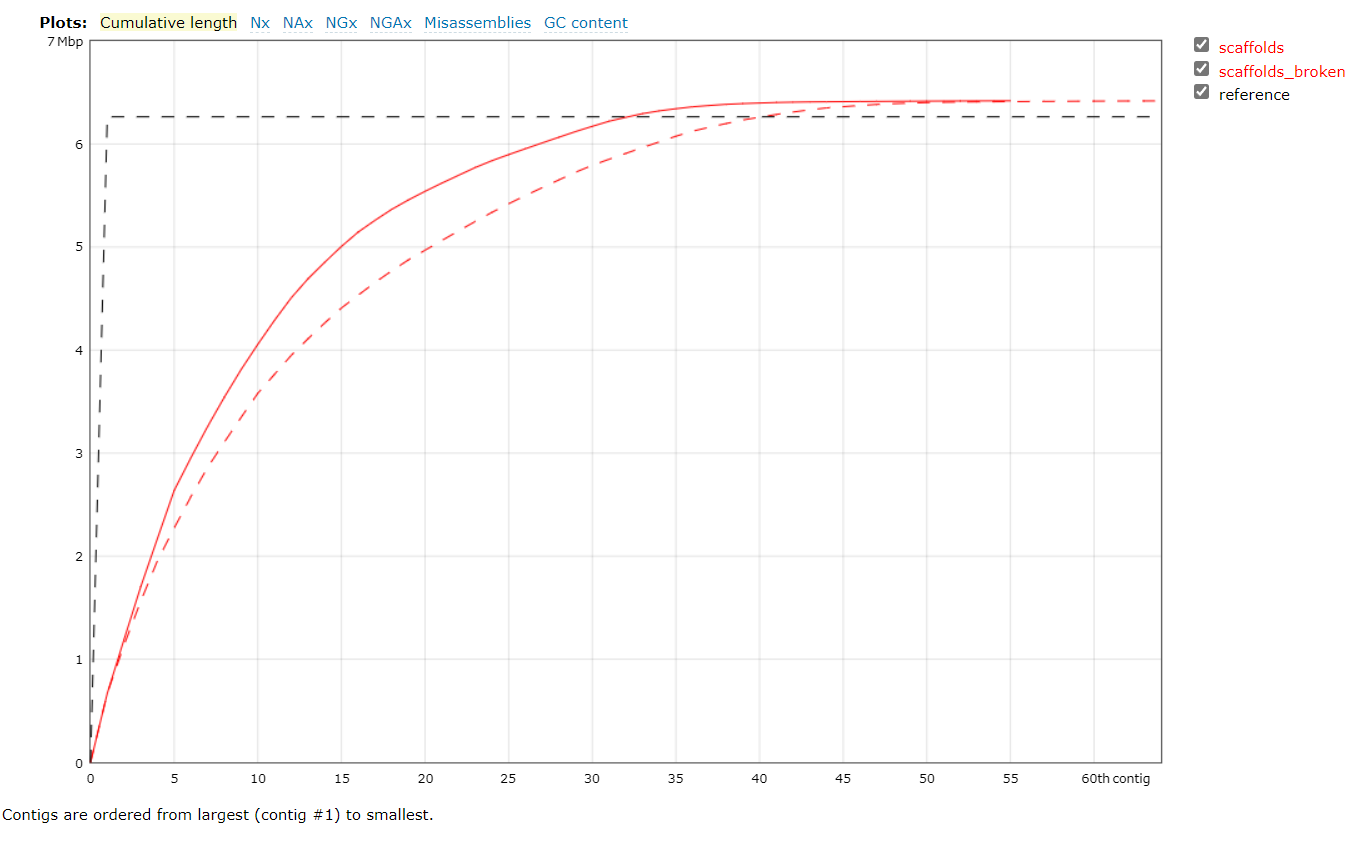
\includegraphics[width=9cm]{imagenes/mapeocon.png}
\caption{Gráfica de longitud acumulativa de la calidad con referencia}
\end{figure}

\subsubsection{Anotación}
Aqui se muestran los resultados de la anotación funcional, estrucutral y de manera general de scaffold NODE\_1\_length\_668648\_cov\_39.096881

\paragraph{Anotación estructural}
Después de correr Augustus en su versión web con los parámetros previamente explicados en la sección II-7 se obtuvo el siguiente resultado, a una escala de 25.5kbp

\begin{figure}[H]
\centering
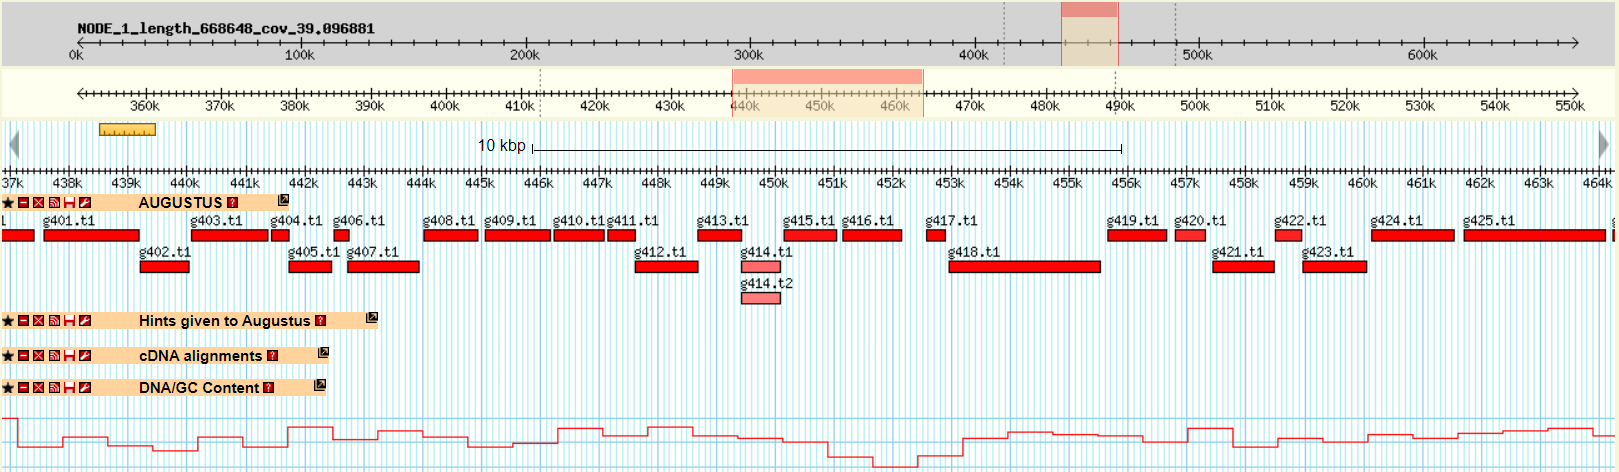
\includegraphics[width=9cm]{imagenes/agugustus.png}
\caption{Anotación estructural por medio de augustus}
\end{figure}

De esta región del scaffold tomamos los genes marcados con los indicadores g401.t1 al g425.1 para que una vez extraídos las secuencias de aminoácidos y nucleótidos del reporte de augustus se procede a realizar la anotación funcional por medio de blast del NCBI y de blast2GO

\paragraph{Anotación funcional}
Al correr Blast con los parámetros explicados en la seccion II-7 se logró encontrar coincidencias de valores mínimos 90\% para los 24 genes estudiados. Dichos reportes por la cantidad de información se anexan en el repositorio, en la carpeta de Análisis funcional 

Al correr el archivo de nucleotidos.fna en Blast2Go y el blast de NCBI se encontraron los siguientes resultados.

\begin{table}[H]
\begin{center}
\caption{Resultados de anotación funcional del Scaffold Node\_1}
\begin{tabular}{|p{1cm}|p{3.5cm}||p{1cm}||p{1cm}|} 
\hline
Nombre Seq & Descripción & Longitud & \%Identidad \\ \hline
g401.t1 & CTP synthase & 1629 & 100\% \\ \hline
g402.t1 & 3-deoxy-8-phosphooctulonate synthase & 846 & 99\% \\ \hline
g403.t1 & phosphopyruvate hydratase & 1290 & 99\% \\ \hline
g404.t1 & cell division protein FtsB & 285 & 99.84\%  \\ \hline
g405.t1 & 2-C-methyl-D-erythritol 4-phosphate cytidylyltransferase  & 705 & 99\%  \\ \hline
g406.t1 & sulfurtransferase-like selenium metabolism protein YedF & 249 & 98\%  \\ \hline
g407.t1 & selenium metabolism membrane protein YedE/FdhT [Pseudomonas aeruginosa] & 1227 & 99.75\%  \\ \hline
g408.t1 & glutathione-dependent formaldehyde neutralization regulator & 909 & 99\%  \\ \hline
g409.t1 & S-(hydroxymethyl)glutathione dehydrogenase/class III alcohol dehydrogenase & 1113 & 99\%  \\ \hline
g410.t1 & S-formylglutathione hydrolase & 852 & 99\%  \\ \hline
g411.t1 & 2-C-methyl-D-erythritol 2,4-cyclodiphosphate synthase & 474 & 99\%  \\ \hline
g412.t1 & tRNA pseudouridine(13) synthase TruD & 1068 & 99\%  \\ \hline
g413.t1 & 5'/3'-nucleotidase SurE & 640 & 99\% \\ \hline
g414.t1 & O-methyltransferase & 672 & 99\% \\ \hline
g414.t2 & O-methyltransferase & 669 & 99\% \\ \hline
g415.t1 & peptidoglycan DD-metalloendopeptidase family protein  & 894 & 99\% \\ \hline
g416.t1 & RNA polymerase sigma factor RpoS & 1005 & 99\% \\ \hline
g417.t1 & ferredoxin family protein & 324 & 100\% \\ \hline
g418.t1 & DNA mismatch repair protein MutS & 2568 & 100\% \\ \hline
g419.t1 & TolB family protein  & 1008 & 91\% \\ \hline
g420.t1 & CinA family protein & 507 & 99\% \\ \hline
g421.t1 & recombinase RecA  & 1041 & 96\% \\ \hline
g422.t1 & recombination regulator RecX & 462 & 99\% \\ \hline
g423.t1 & LOG family protein & 1071 & 99\% \\ \hline
g424.t1 & MBL fold metallo-hydrolase & 1404 & 97\% \\ \hline
g425.t1 & xylulose 5-phosphate 3-epimerase & 2406 & 99\% \\ \hline
\end{tabular}
\end{center}
\end{table}


\begin{figure}[H]
\centering
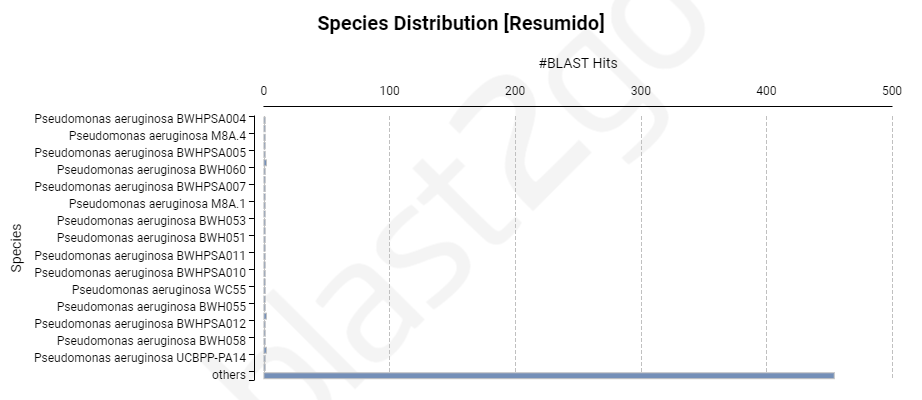
\includegraphics[width=9cm]{imagenes/species_distribution.png}
\caption{Distribución de especies}
\end{figure}

\begin{figure}[H]
\centering
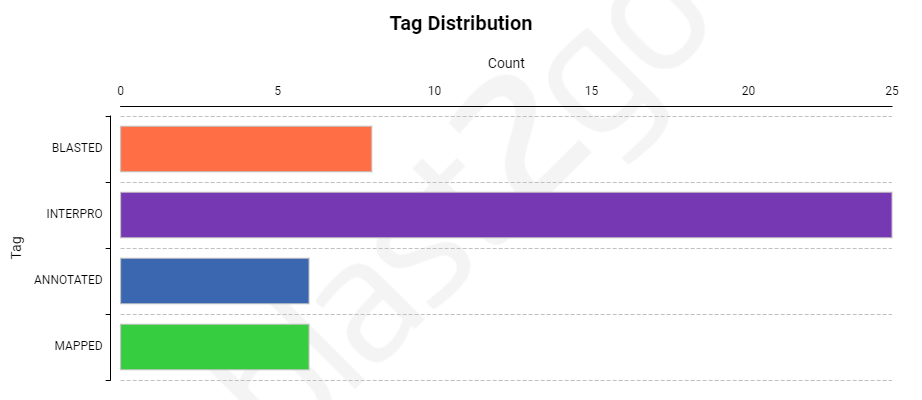
\includegraphics[width=9cm]{imagenes/tag_distribution.png}
\caption{Resultados de blast2GO en histograma de distribución}
\end{figure}



\section{Discusiones y conclusiones}
A partir del análisis de calidad inicial podemos comprobar que la calidad del archivo 2 pareado es inferior al archivo 1, aun así, con el filtrado de fast pig pudimos poco más de 300,000 secuencias que no cumplían un mínimo de calidad de phred 30, Así como eliminar los adaptadores. Del ensamble del genoma podemos observar en el cuadro 2 Que el total de la longitud es similar al del valor de la referencia Siendo de 6419571 para nuestro ensamble contra 6264404, Asimismo también es similar el valor del porcentaje de GC, siendo de 66.39 de nuestro mapeo contra 66.56 del valor de la referencia. Tenemos un total de 80 scaffolds siendo poco menos de la mitad, 38 mayores o iguales a 10000bp. Por lo que podemos concluir que el ensamble es confiable para realizar la anotación dada la similitud con la referencia.
En la anotación estudiamos 26 genes del primer scaffold  Scaffold Node\_1 , del g401.t1 al g425.t1,  de los cuales 25 presentan un solo alelo y gen g414 presenta  2 alelos del mismo en nuestro organismo de estudio g414.t1 y g414.t2 respectivamente, y al momento de realizar la anotación funcional mediante BLAST y blast2GO vemos que efectivamente cumplen la misma función que es codificar para O-methyltransferase, y tiene una diferencia de longitud de apenas 3 nucleótidos. Del resto de la anotación podemos decir que en base a los porcentajes de identidad que van del 91\% al 100\% en los genes estudiados esa región del scaffold es muy acordé a lo que se espera en las referencias de las bases de datos. Asimismo, de las gráficas de blast2GO podemos observar que la distribución de especies todas aparecen como \textit{pseudomonas aeruginosa} pero hay un error que aparece como otros, el cual apareció después de terminar de anotar mediante este software por lo que se lo atribuyo un error de configuración ya que sólo 7 genes de los 26 estudiados pudieron completar el blast solamente 6 pudieron mapearse y anotarse. Aun así, la información que arrojó Blast del me permitió llegar al cuadro III en el cual está la descripción de que codifican cada uno de los 26 genes estudiados así como su longitud y porcentaje de similitud arrojado por el Blast.


\appendices
\section{Descripción de herramientas bioinformáticas usadas.}
\begin{itemize}
\item SRAtoolkit : Es un conjunto de herramientas proporcionadas por el NCBI para poder descargar secuencias de la base de datos de Sequence Read Archive (SRA) data
\item FastQC : Proporcionar una forma sencilla de realizar algunas comprobaciones de control de calidad en los datos de secuencia sin procesar que provienen de piplines de secuenciación de alto rendimiento. Es una manera rápida y sencilla de usar de realizar comprobaciones de calidad.
\item FastP : Herramienta para procesar datos de FASTQ, El algoritmo tiene funciones para control de calidad, recorte de adaptadores, filtrado por calidad y poda de lectura. 
\item bowtie2 : Herramienta para realizar mapeos de secuencaicion mediante el uso de referencias. Bueno para alinear lecturas de aproximadamente 50 hasta 100 o 1,000 caracteres, y particularmente bueno para alinearse con genomas relativamente largos. Funciona mediante la creación de un indice de referencia
\item FAS Center for Systems Biology : Plataformade la Universidad de Harvard que contiene varios scriptos escritos en Perl para el procesamiento de datos biológicos, principalmente en formato FASTA
\item SPAdes : Es un ensamblador de genomas diseñado para genomas relativamente pequeños. Principalmente para bacterias.
\item Augustus : Es un programa que predice genes de una secuencias genómicas. Es de código abierto, y funciona para la anotación estructural
\item Blast2GO : Es un programa propietario para realizar de manera automática la anotación funcional de datos de secuencias genómicos. Se apoya principalmente del algoritmo de BLAST
\item BLAST : Basic Local Alignment Search Tool (BLAST) es una herramienta que permite encontrar similitud de secuencias ya sea de nucleótidos o de proteínas. Lo hace con el apoyo de varias bases de datos de secuencias y se puede utilizar para inferir la anotación funcional y evolutiva de secuencias.
\end{itemize}


\begin{thebibliography}{7}

\bibitem{IEEEhowto:kopka}
Nachtweide, S., \& Stanke, M. (2019). Multi-Genome Annotation with AUGUSTUS. Methods in Molecular Biology (Clifton, N.J.), 1962, 139–160.  \url{ https://doi.org/10.1007/978-1-4939-9173-0_8}

\bibitem{IEEEhowto:kopka}
Langmead, B., \& Salzberg, S. L. (2012). Fast gapped-read alignment with Bowtie 2. Nature Methods, 9(4), 357.  \url{ https://doi.org/10.1038/NMETH.1923}

\bibitem{IEEEhowto:kopka}
Langmead, B., Wilks, C., Antonescu, V., \& Charles, R. (2019). Scaling read aligners to hundreds of threads on general-purpose processors. Bioinformatics, 35(3), 421–432.  \url{ https://doi.org/10.1093/BIOINFORMATICS/BTY648}

\bibitem{IEEEhowto:kopka}
Stover, C. K., Pham2, X. Q., Erwin, A. L., Mizoguchi, S. D., Warrener, P., Hickey, M. J., Brinkman3, F. S. L., Hufnagle, W. O., Kowalik, D. J., Lagrou, M., Garber, R. L., Goltry, L., Tolentino, E., Westbrock-Wadman, S., Yuan, Y., Brody, L. L., Coulter, S. N., Folger, K. R., Kas2, A., … Olson2, M. v. (2000). Complete genome sequence of Pseudomonas aeruginosa PAO1, an opportunistic pathogen. NATURE, 406.  \url{www.nature.com}

\bibitem{IEEEhowto:kopka}
Bankevich, A., Nurk, S., Antipov, D., Gurevich, A. A., Dvorkin, M., Kulikov, A. S., Lesin, V. M., Nikolenko, S. I., Pham, S., Prjibelski, A. D., Pyshkin, A. v., Sirotkin, A. v., Vyahhi, N., Tesler, G., Alekseyev, M. A., \& Pevzner, P. A. (2012). SPAdes: A new genome assembly algorithm and its applications to single-cell sequencing. Journal of Computational Biology, 19(5), 455–477.  \url{https://doi.org/10.1089/CMB.2012.0021}

\bibitem{IEEEhowto:kopka}
Lantz, H., Dominguez Del Angel, V., Hjerde, E., Sterck, L., Capella-Gutierrez, S., Notredame, C., Vinnere Pettersson, O., Amselem, J., Bouri, L., Bocs, S., Klopp, C., Gibrat, J. F., Vlasova, A., Leskosek, B. L., Soler, L., \& Binzer-Panchal, M. (2018). Ten steps to get started in Genome Assembly and Annotation. F1000Research, 7. \url{https://doi.org/10.12688/F1000RESEARCH.13598.1}

\bibitem{IEEEhowto:kopka}
Chen, S., Zhou, Y., Chen, Y., \& Gu, J. (2018). fastp: an ultra-fast all-in-one FASTQ preprocessor. Bioinformatics, 34(17), i884–i890.  \url{https://doi.org/10.1093/BIOINFORMATICS/BTY560}


\end{thebibliography}



\end{document}


